
\section{Wu-Experiment}

\chapterauthor{Inga Höfmann, 02.11.2018}

\subsection{Historische Entwicklung}
Das Wu-Experiment beschäftigt sich mit der Parität, welche als Operator eine Inversion in allen Raumkoordinaten beschreibt. Es gilt
\begin{align*}
	\hat{P} \vec{r} &= -\vec{r}, &
	\hat{P} \vec{L} &= \vec{L}.
\end{align*}
Die Parität wurde erstmals im Jahre 1927 als Quantenzahl und somit intrinsische Eigenschaft eines Teilchen eingeführt und galt zunächst für alle Wechselwirkungen als erhalten.
Zweifel an der Parität als Erhaltungsgröße kamen im Jahr 1954 mit dem sogenannten $\tau$-$\theta$-Puzzle auf:
Die damals als $\tau$- und $\theta$-Meson bekannten Teilchen besaßen identische Massen, Ladungen und Lebensdauern.
Unterschiede ergaben sich lediglich in den Zerfallsprodukten:
Während das $\tau^+$-Meson in den Endzustand $\pi^+ \pi^+ \pi^-$ (Parität $-1$) zerfiel, war der Endzustand des $\theta^+$-Mesons $\pi^+ \pi^0$ (Parität $+1$).
Als Erklärung dieses Puzzles existierte die Möglichkeit, dass es sich bei beiden Mesonen um das gleiche Teilchen handelt und die Parität in diesem Fall verletzt ist.
Diese Vermutung wurde, zusammen mit Vorschlägen für einen experimentellen Aufbau, im Jahre 1957 von Tsung-Dao Lee und Chen Ning Yang in einem Paper veröffentlicht, wofür sie 1957 den Nobelpreis erhielten.
Das dazugehörige Experiment wurde von der Physikerin Chien-Shiung Wu im Jahre 1956 innerhalb von neun Monaten realisiert.

\subsection{Idee des Wu-Experimentes}
Die Idee des Wu-Experimentes ist es, eine Paritätsverletzung in der schwachen Wechselwirkung nachzuweisen.
Um einen Interferenzterm mit paritätserhaltenden und paritätsverletzenden Anteilen untersuchen zu können muss eine pseudoskalare Messgröße genutzt werden.
Hierzu bietet es sich an, die Winkelverteilung $I\left(\theta \right)$ von $e^-$ in einem $\beta$-Zerfall zu betrachten. 
Es ergibt sich ein Parameter $\alpha$, welcher die Asymmetrie in der Winkelverteilung beschreibt, wobei $\alpha = 0$ für Paritätserhaltung bzw. $\alpha \neq 0$ für Paritätsverletzung gilt.

Das Wu-Experiment ist so konzipiert, dass es rein qualitative Aussagen über den Parameter $\alpha$ treffen kann.
Als Probe wird $\ce{^{60}_{27}Co}$ verwendet, welches dominant unter Aussendung eines $e^-$ und eines $\bar{\nu_e}$ (d.h. unter der schwachen Wechselwirkung) in $\ce{^{60}_{28}Ni^{*}}$ zerfällt. Dieses sendet wiederum zwei energetisch charakteristische Photonen aus um in einen nicht angeregten Zustand zu gelangen.
Zu beachten ist, dass $\ce{^{60}_{27}Co}$ einen Spin von $5$ und $\ce{^{60}_{28}Ni^{*}}$ einen Spin von $4$ besitzt.
Somit müssen die Ausrichtungen der Spin-$z$-Komponente des $e^-$, des $\bar{\nu_e}$ (beide mit Spin $\sfrac{1}{2}$) und des $\ce{^{60}_{28}Ni^{*}}$ alle in die gleiche Richtung zeigen.
Werden die Spins der Kobalt-Atome nun in eine Vorzugsrichtung ausgerichtet, kann die Anzahl der Elektronen in Spinrichtung gemessen werden.
Wird die Vorzugsrichtung der Spins umgekehrt, was einer Paritätstransformation entspricht, so wird die Anzahl der Elektronen gegen die Spinrichtung gemessen.
Somit wird die Messung einer möglichen Paritätsverletzung ermöglicht.

\subsection{Experimentelle Herausforderungen}
Insbesondere die Ausrichtung der Spins der Kobalt-Atome stellt eine große experimentelle Herausforderung dar.
Hierfür werden sowohl sehr geringe Temperaturen ($\approx \SI{1}{\kelvin}$) als auch hohe Magnetfelder ($\approx \SI{10}{\tesla}$) benötigt.
Die Lösung stellte die sogenannte Rose-Gorter-Methode dar.
Hierbei wird ein Kristall, $\ce{CeMg}$-Nitrat, verwendet, wobei das Salz einen anisotropen $g$-Faktor besitzt.
Die starke Abkühlung geschieht durch das Anlegen eines B-Feldes entlang des maximalen $g$-Faktors.
Zunächst werden dabei die, aufgrund der Hyperfeinstrukturaufspaltung entstehenden, niedrigeren Energieniveaus besetzt.
Anschließend wird das System thermisch isoliert und das Magnetfeld heruntergefahren.
Durch diese sogenannte adiabatische Entmagnetisierung können hinreichend geringe Temperaturen erreicht werden.
Das Anlegen eines Magnetfeldes in Richtung des minimalen $g$-Faktors ermöglicht dann die Polarisation der Hüllenelektronen des Kobalts.
Dies führt zu einer starken Zunahme des $B$-Feldes in der Nähe des Kerns und somit zu einer Polarisation der Spins der Kerne.
Werte der Polarisation von bis zu $\SI{60}{\percent}$ konnten hiermit erreicht werden.
Die experimentelle Realisierung ist in Abbildung \ref{fig:wu} dargestellt.

\begin{figure}
  \centering
  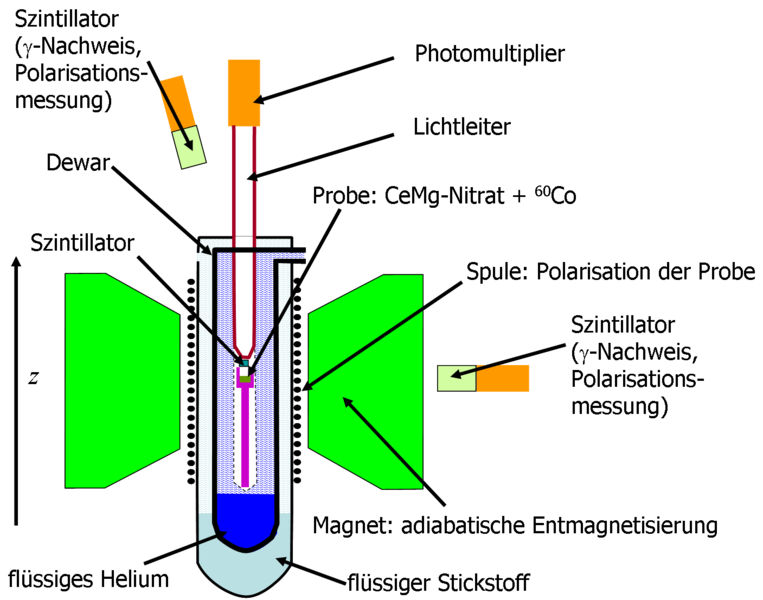
\includegraphics[height=7.0cm]{ressources/wu.png}
  \caption{Schematischer Aufbau des Wu-Experimentes \cite{wu}.}
  \label{fig:wu}
\end{figure}

Die Polarisation des Kernspins geschieht über die $\gamma$-Szintillatoren, da die Photonen vorzugsweise in Spin-Richtung emittiert werden.
Der Nachweis der Elektronen geschieht direkt über den Szintillatorkristall über Photomultiplier.
Um die Parität untersuchen zu können wird das gesamte Experiment mit zwei verschiedenen Ausrichtungen des Magnetfeldes und somit mit zwei verschiedenen Vorzugsrichtungen der Spins durchgeführt.

\subsection{Experimentelle Ergebnisse und Konsequenzen}
Experimentell konnte nachgewiesen werden, dass die Kernspins hinreichend polarisiert werden konnten.
Zudem wurde gezeigt, dass die Elektronen vorzugsweise gegen die Richtung des Kernspins des Kobalts emittiert werden.
Dies entspricht einer Verletzung der Parität und bestätigte somit die These von Tsung-Dao Lee und Chen Ning Yang.
Spätere Experimente wiesen quantitativ nach, dass die Parität tatsächlich maximal verletzt ist.
Zudem folgte die theoretische Erkenntnis, dass die schwache Wechselwirkung eine V-A-Struktur besitzt:
Sie koppelt nur an linkshändige Teilchen und rechtshändige Antiteilchen, was die maximale Paritätsverletzung erklärt.

\subsection{Diskussion zum Vortrag}
Als Frage wurde gestellt, ob die Suche nach Paritätsverletzung in anderen Wechselwirkungen ebenfalls durchgeführt wurde.
Hierbei ergab sich die Antwort, dass bis heute nach paritätsverletzenden Anteilen außerhalb der schwachen Wechselwirkung gesucht wird.

Da Kobalt zwei unterschiedliche $\beta^-$-Zerfallsmoden in Nickel besitzt, kam die Frage auf wie diese Unterschiede experimentell berücksichtigt wurden.
Dies war möglich und wurde realisiert, da die Szintillatoren auf die festen Energien der Photonen ausgerichtet werden können.

Zuletzt wurde über technische Details der Kühlung diskutiert.
Hierbei wurde das Pumpen erwähnt, welches genutzt wurde, um eine Kühlung auf bis zu $\SI{1}{\kelvin}$ zu ermöglichen.
